\section{Validatie en kalibratie}
Als de applicatie ontworpen is en gemaakt. Is het nodig om dit te valideren en waar nodig te kalibreren en trimmen.
\subsection{Energie verbruik}
Voor de applicatie is in Paragraaf \ref{Block_schema}: Blokschema niveau een verdeling gemaakt over het energieverbruik. Uit testen blijkt dat het vermogen anders is verdeeld. Dat is in Tabel \ref{tab:Energie_verbruik_validatie} weergegeven.

\begin{table}[H]
    \centering
    \begin{tabular}{|c|c|}
        \hline
        \textbf{Blokken} & \textbf{Energie verbruik} \\ \hline
        Temperatuur sensor \& anti aliasing filter & 0,94 mW \\ \hline
        Versterker temperatuur sensor  & 65 $\mu$W \\ \hline
        Digitale signaal bewerking & 1,41 mW \\ \hline
        Relatieve luchtvochtigheid sensor & 1,32 $\mu$W \\ \hline
        Zend module & 0.44 mW \\ \hline
        totaal  & 2.857 mW \\ \hline
    \end{tabular}
    \caption{Vermogens verdeling van de applicatie gemeten.}
    \label{tab:Energie_verbruik_validatie}
\end{table}
Uit deze meetwaardes is gebleken dat het verbruik van de applicatie binnen specificaties valt.

\subsection{Relatieve luchtvochtigheid sensor}
Voor het meten en valideren van de relatieve luchtvochtigheid wordt er gebruik gemaakt van een relatieve luchtvochtigheid sensor die intern een kalibratie rapport heeft, zodat hij beter is dan wat onze specificatie verwacht. Om ervoor te zorgen dat de informatie van beide sensoren klopt, wordt er gebruik gemaakt van een klimaat kamer. Dit wordt gedaan met behulp van een klimaatkamer en een SHT85 (validatie sensor). De sensor is getest van 0 procent tot 90 procent bij een temperatuur van 20 graden Celsius. De meetresultaten zijn weergegeven in Figuur \ref{fig:meet_result_luchtvochtigheid}. Hierin is zichtbaar dat de sensor altijd onder de twee procent afwijking blijft. Hiermee is bepaald dat de sensor binnen specificaties valt.

\begin{figure}[H]
    \centering
    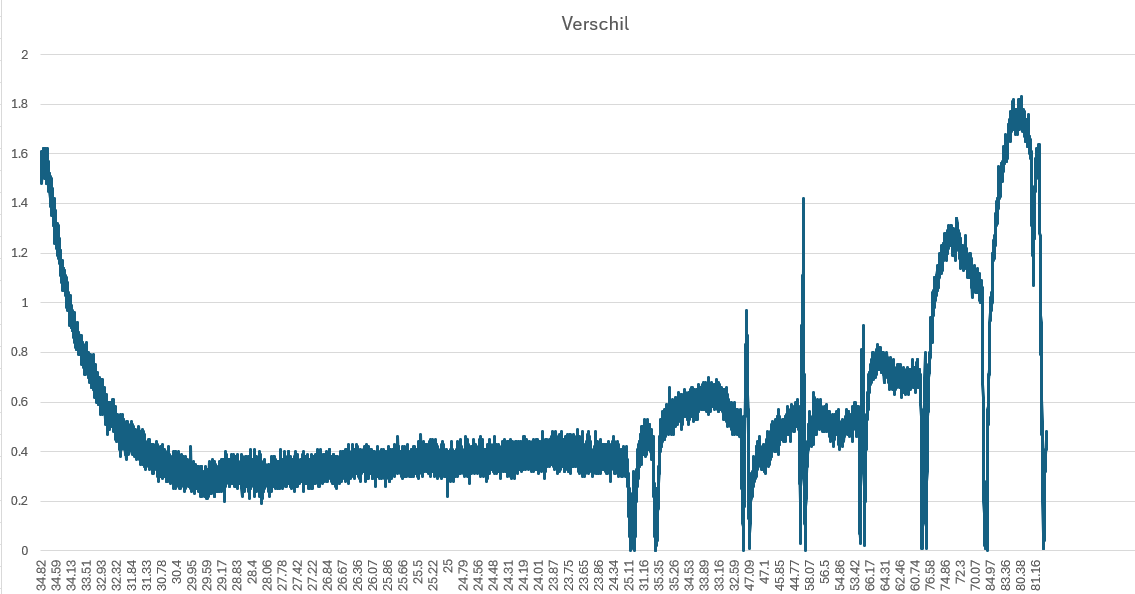
\includegraphics[width=0.75\linewidth]{pictures/meetresultaten_luchtvochtigheid.png}
    \caption{Het verschil tussen de sensor en validatie sensor in procenten weergegeven.}
    \label{fig:meet_result_luchtvochtigheid}
\end{figure}

\subsection{Temperatuur sensor}
Voor het meten en valideren van de temperatuur wordt er gebruik gemaakt van een van een temperatuur sensor die intern een kalibratie rapport heeft. Hierdoor kan de sensor gebruikt worden om onze eigen ontwikkelde sensor te valideren. Voor het meten moet dit gedaan worden in een ruimte waar de temperatuur gecontroleerd is. Dit wordt gedaan met behulp van een klimaatkamer en een SHT85 (validatie sensor). De sensor is getest van -4 tot 11 graden Celsius. Het testen van het verdere bereik van de sensor was helaas niet mogelijk, omdat de klimaatkamer kapot ging. Hierdoor is het niet gelukt om een volledige trim en kalibratie te maken voor het hele bereik. Maar is er wel een trim en kalibratie functie ontworpen voor het bereik dat gemeten is. De gemeten waardes zijn weergegeven in Figuur \ref{fig:meet_result_temp_sensors}. Deze data is daarna gefilterd om meet fouten uit te sluiten en is door een polynoom functie getrimd en heeft daar daarom nog maar een afwijking van 0,1 graden Celsius. Dit is weergegeven in Figuur \ref{fig:trim_resulaten_temp_sensor}.
\begin{figure}[H]
    \centering
    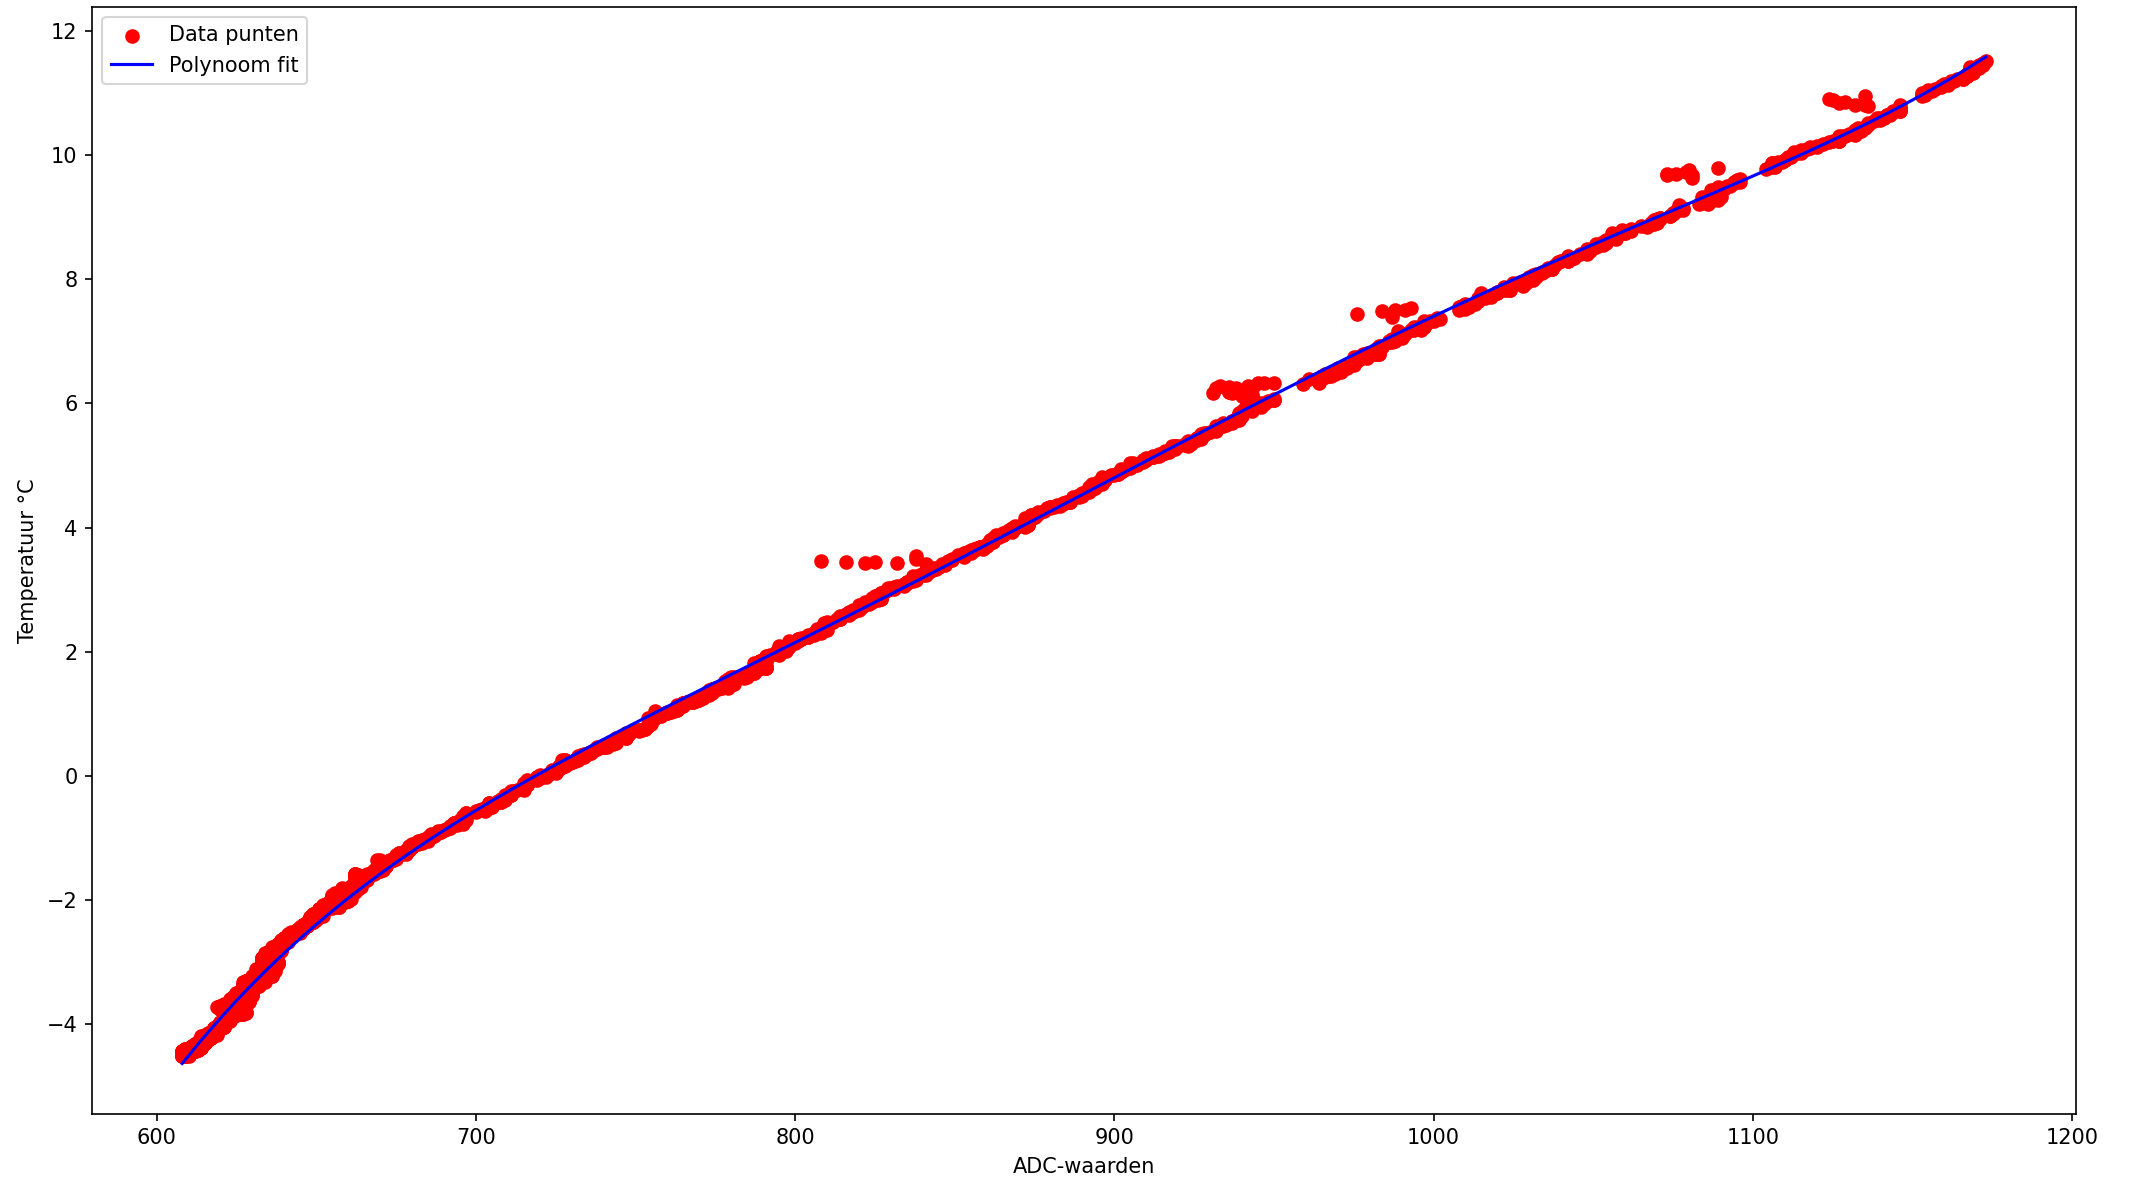
\includegraphics[width=0.75\linewidth]{pictures/meet_resultaten_temp_sensor.png}
    \caption{Meetresultaten van de temperatuur sensor ten opzichte van de validatie sensor.}
    \label{fig:meet_result_temp_sensors}
\end{figure}

\begin{figure}[H]
    \centering
    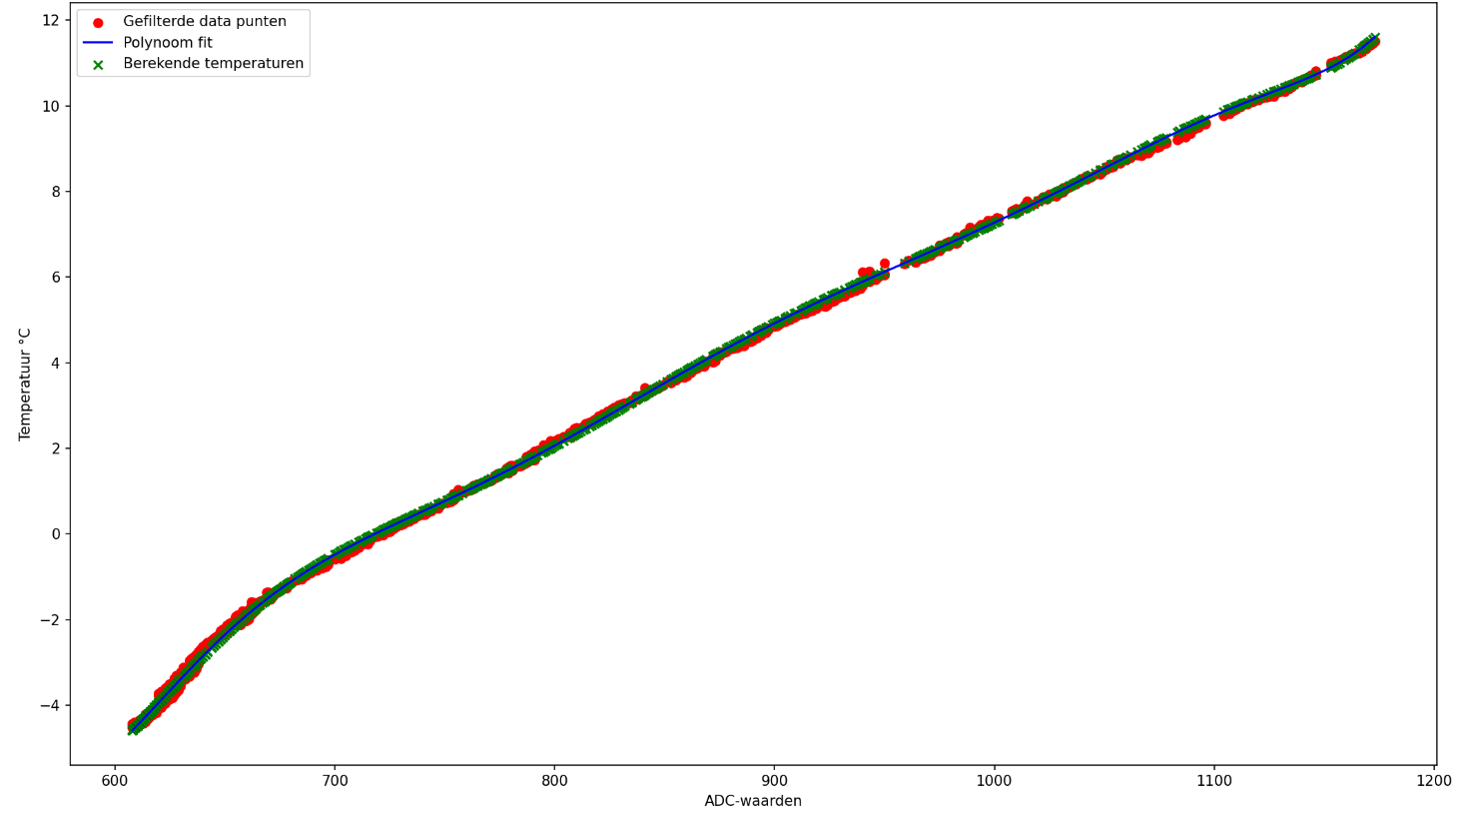
\includegraphics[width=0.75\linewidth]{pictures/trim_resultaten_temp_sensor.png}
    \caption{Getrimde resultaten van de temperatuur sensor ten opzichte van de validatie sensor. }
    \label{fig:trim_resulaten_temp_sensor}
\end{figure}